% !Mode:: "TeX:UTF-8"
\chapter{研究现状}

对象操纵是 VR 技术中最为基本且必要的交互行为之一。针对对象操纵这一特定的研究主题,扩展现实的所有门类,甚至传统计算机图形界面的研究成果皆可启发虚拟现实的更新和发展。在过去的二十年里,国内外许多相关领域学者致力于对象操纵的相关研究。根据已有的研究内容,扩展现实中的对象操纵方法主要由以下三大思想构成:(1)基于手部(含手柄)动作;(2)基于语音;(3)基于眼动\upcite{2018Mendes}\upcite{2020Jaziar}。

\section{基于手部(含手柄)的操纵}

\begin{figure}[b!]
    \centering
    \subfigure[PRISM]{
        \label{fig-1-l}
        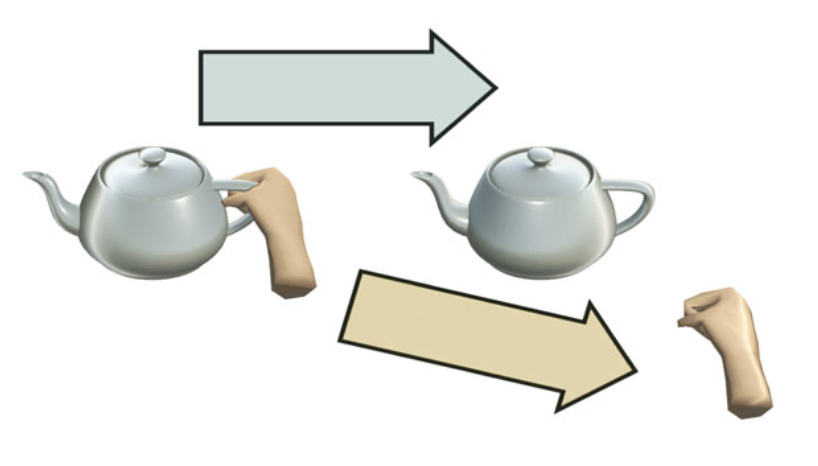
\includegraphics[width=.32\textwidth]{figure/prism.png}
    }
    \hspace{2em} % 水平间隔
    \subfigure[Go-Go]{
        \label{fig-1-m}
        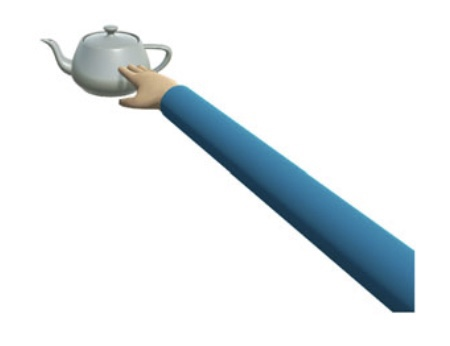
\includegraphics[width=.22\textwidth]{figure/gogo.jpg}
    }
    \hspace{2em} % 水平间隔
    \subfigure[射线广播]{
        \label{fig-1-r}
        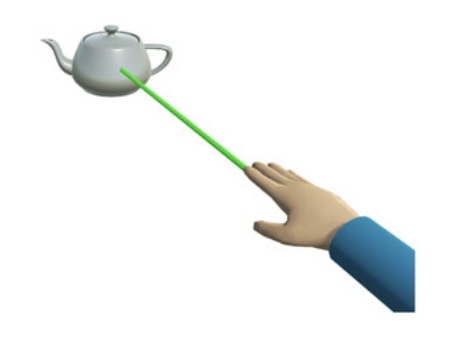
\includegraphics[width=.22\textwidth]{figure/raycasting.jpg}
    }
    \caption{研究早期三种主要的基于手部动作追踪的对象操纵方法}
    \label{fig-1}
\end{figure}

在基于手部(含手柄)追踪的方法研究早期,学界主要的三大思路为在虚拟环境中单手直接操纵、延长用户手臂和射线广播(ray-casting),见图\ref{fig-1}。虚拟延长手臂思路的代表研究来自于Ivan Poupyrev团队在1996年发表的Go-Go沉浸式交互方法\upcite{1996Poupyrev}。Go-Go使用交互式增长用户手臂的元函数和非线性映射来指定和操纵远处的物体。与同时期的其他技术不同的是,Go-Go允许对附近的和远处的物体进行无缝直接操纵。然而,Go-Go技术提出的物体选择和操控模式并不能完全作为一个完整的交互方法来供人们使用; Go-Go应该被视为以同时期技术为基础的一个补充,而不能完全取而代之。射线广播的思路和虚拟延长手臂类似;射线广播的思路是将射线束从使用者的手中延伸出来,从而指定操纵物体。然而,射线广播思路存在比较明显的弊端。由于在射线广播的对象操纵中物体是被连接到射线末端的,所以除了以射线本身为轴可以完成的动作,许多操纵都是难以简单实现的,因为只有一个自由度(围绕射线轴的旋转)可以用射线广播的方式独立控制。比如,若用户希望以与射线方向垂直的轴向旋转一个物体,单纯以射线广播是无法完成的。此外,射线广播还缺乏一种控制物体与用户之间距离的方法,导致用户无法准确地将物体拉近或推远,而这也是对象操纵的基础功能之一。

当把Go-Go方法和射线广播以及其他方法(例如通过将虚拟手臂延伸到无限远来改进Go-Go的Stretch Go-Go)进行比较时,并没有明显的赢家\upcite{1997Doug}。用户评估结果显示,所有技术都有明显的缺点。在这次评估中,HOMER方法被提出来了;这是一种以手为中心的基于射线广播的对象操作技术\upcite{1997Doug}。HOMER使用射线来选择物体,在选择物体后,它将虚拟的手移动到物体上;用户的身体和手之间的当前距离被映射为到虚拟物体的距离。因此,HOMER方法操纵对象的方式与Go-Go技术类似,但缩放系数是针对每个选定的物体独立计算的。

\begin{figure}[t!]
    \centering
    \subfigure[基于双手直接操纵的Z技术]{
        \label{fig-2-u}
        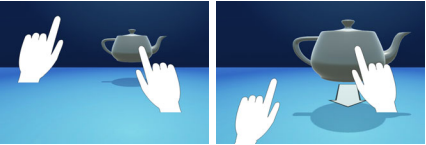
\includegraphics[width=.45\textwidth]{figure/z_technique.png}
    }
    \subfigure[基于双手直接操纵的Sticky Tools方法]{
        \label{fig-2-d}
        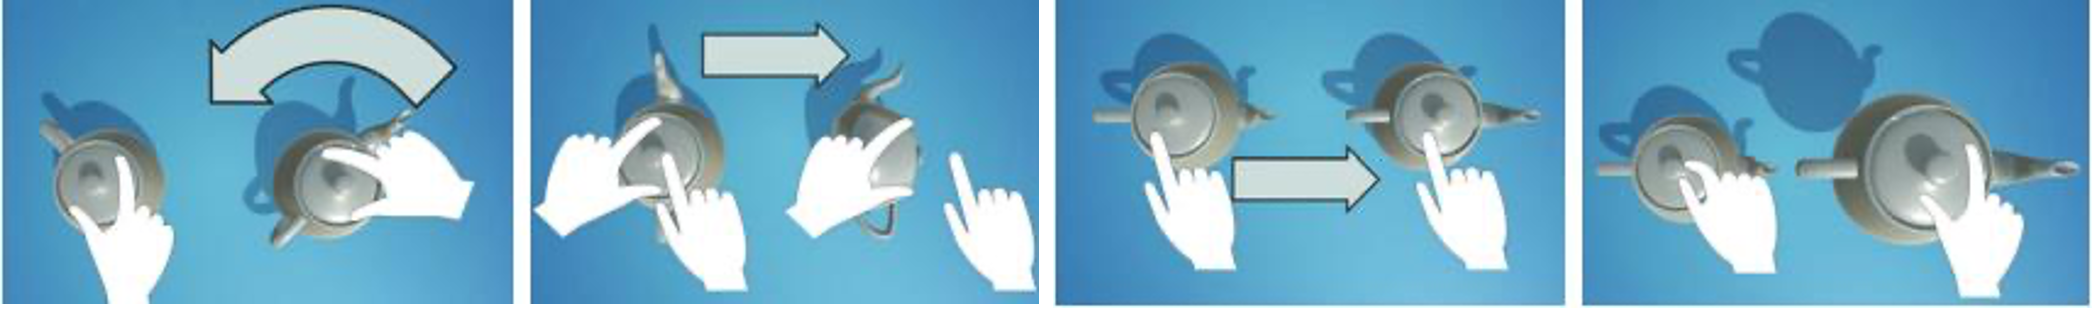
\includegraphics[width=.9\textwidth]{figure/sticky.png}
    }
    \caption{两种具代表性的基于双手动作的对象操纵方法}
    \label{fig-2}
\end{figure}

到了21世纪,学界将研究重心放在虚拟环境对象操纵的精确性上。一个具有代表性的方法是Scott Frees团队在2005年提出的PRISM\upcite{2005Frees},(见图\ref{fig-1-l})PRISM是一种通过缩放操作进行精确和快速交互的方法,它在同时期是一种非常新颖且具有开创性的交互技术。PRISM主动根据用户在虚拟环境中的行为特征来确定他们所想的操纵目标是明确还是不明确的。当操纵目标明确时,PRISM动态地调整“控制/显示”比例来提高对象操纵的精确度。该比例决定了物理手部运动和受控虚拟物体运动之间的关系,降低了传感器对手部运动监测不必要的灵敏度,从而减少操作误差。使用PRISM,用户始终完全控制着被操纵物体的位置。与像Go-Go这样的技术相比,PRISM在能力范围上也有很大提升,最明显的进步在于PRISM扩大了手部运动的规模以允许“远距离”操纵,同时在特定情形中可以主动缩小手部运动的幅度以提高精确度。

在这之后,Curtis Wilkes等人将PRISM与HOMER相结合,在2008年提出了融合了两种方法精华的Scaled HOMER\cite{2008Curtis}。Scaled HOMER使用基于速度的缩放,允许用户在近距离和远距离进行更为精确的操作。它比原始的HOMER在各种任务条件下,尤其是有关需要高度精确、远距离放置物体或大运动距离的任务中的性能都有所提高。2015年,在Go-Go和PRISM研究之后,Chris Auteri等人将这两种技术结合起来,以提高延伸的三维操作的精确性\upcite{2015Auteri}。该方法首先将PRISM直接应用于用户的手(基础光标)的运动,从而基于运动速度计算出一个新的光标位置(PRISM光标)。然后,PRISM光标移动的距离被基于Go-Go距离的启发式方法所放大。与 PRISM和HOMER的结合一样,Go-Go和PRISM的结合提供了一些改进,尤其是在任务完成的成功率和精细度上。

\begin{figure}[t!]
    \centering
    \subfigure[Houde团队的方法]{
        \label{fig-3-l}
        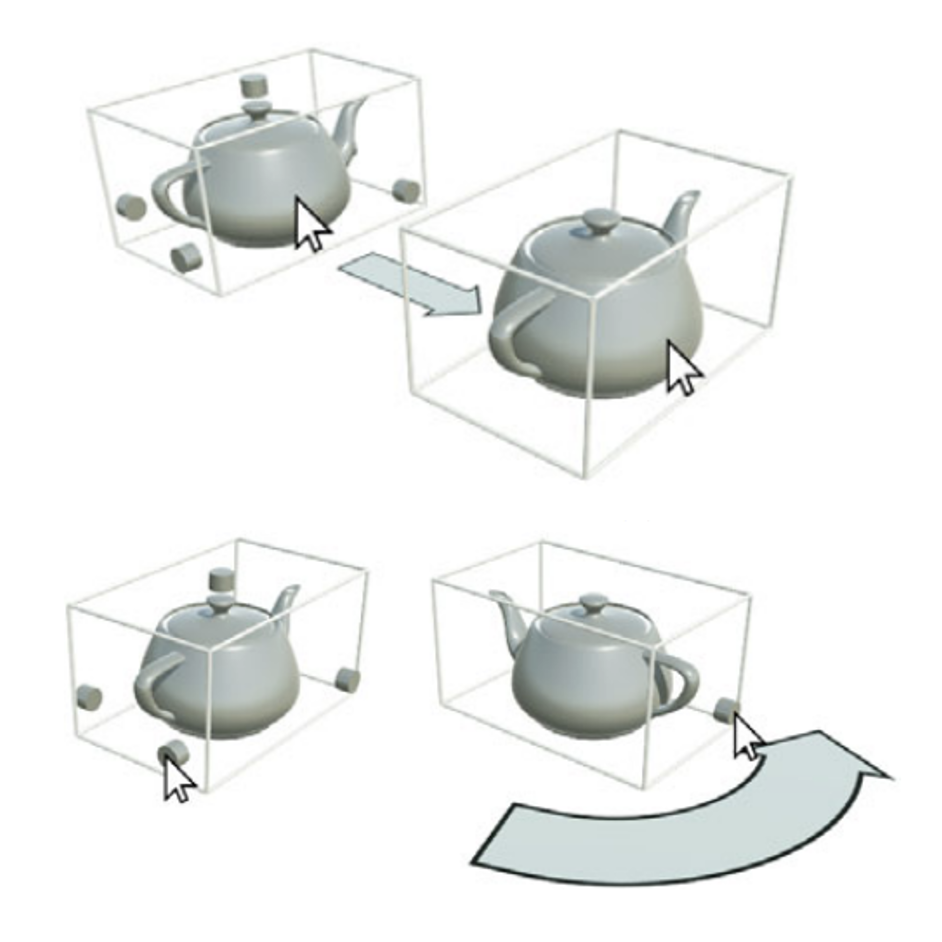
\includegraphics[width=.38\textwidth]{figure/handle_box.png}
    }
    \hspace{5em} % 水平间隔
    \subfigure[Conner团队的方法]{
        \label{fig-3-r}
        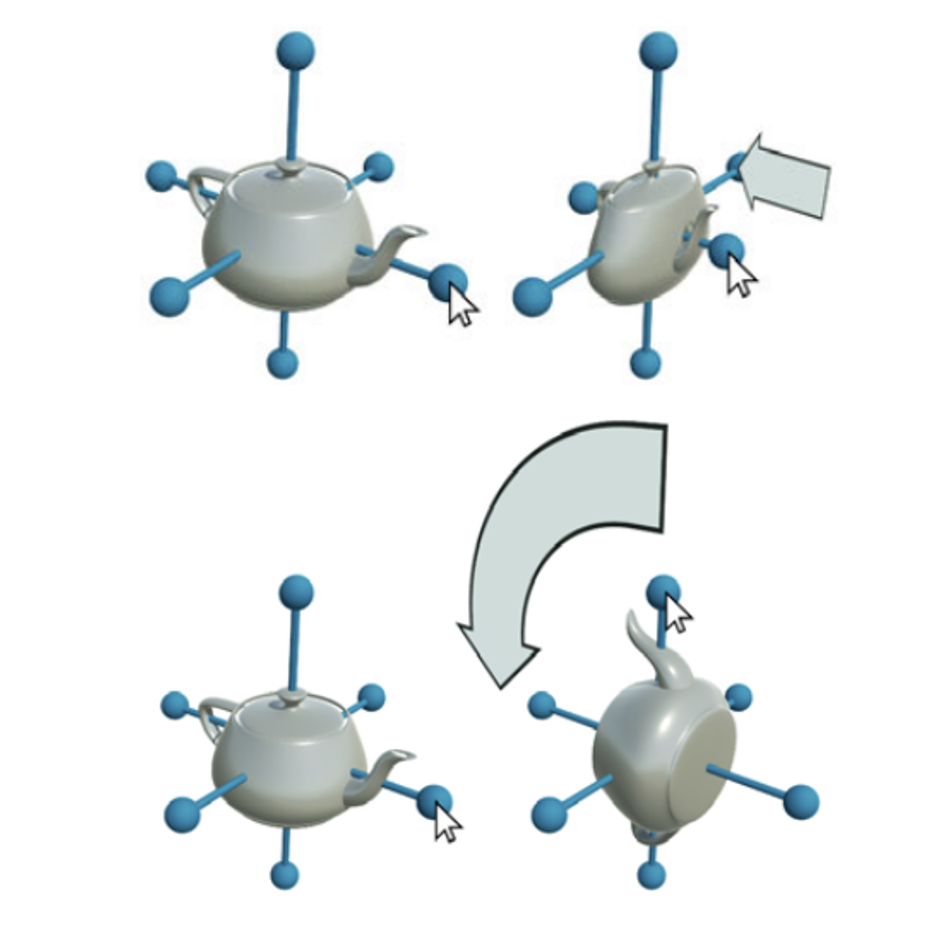
\includegraphics[width=.38\textwidth]{figure/virtual_handles.png}
    }
    \caption{两种具代表性的基于外加虚拟控制柄的对象操纵方法}
    \label{fig-3}
\end{figure}

基于双手的操纵在2008年被Noritaka Osawa团队提出\upcite{2008Noritaka}。该团队提出了一种用于在沉浸式虚拟环境中精确定位3D虚拟物体的单手和双手控制技术。这个方法提出了一种位置调整策略,包括一个类似于PRISM的用于减缓手部运动的比例系数以及一个被动的视角调整。该交互系统会自动将视角接近抓取点,使被操纵的物体看起来更大,从而更易于操控。为了有效控制这些调整,该团队提出了两种技术。第一种是基于单手操纵的;因为当用户想精确地操纵一个物体时,他们的手会慢慢移动,所以通过对单手的速度监测,系统可以判断当前对象是否需要精确操纵。另一种是基于两手间距离的;当用户两手之间的距离很小时,调整就会被激活。通过用户评估,位置和视点的调整比禁用这种调整有更好的操纵效率和用户体验。此外,该团队的测试结果还显示,双手控制比单手表现更好。承接双手直接操纵的方法,Martinet团队提出了两种移动3D对象的技术\upcite{2010Martinet}。第一种扩展了许多CAD(Computer-aided Design,计算机辅助设计)应用程序中的视窗概念;它引入了四个视窗,每个视窗显示3D对象的不同视图。在其中一个视窗中触摸并拖动物体,可以在与该视窗平行的平面上平移物体。第二种方法被称为Z技术;Z技术只使用场景的一个视图(见图\ref{fig-2-u})。在这种技术中,第一次触摸触发在平行于视图的平面上移动物体,第二次触摸触发垂直于视图平面的前后运动。Martinet的初步评估表明,用户更喜欢Z技术。Martinet等人在Z技术的基础上进行了改进,推出了DS3,一种基于DOF分离的三维对象操纵技术\upcite{2010MartinetDOF}。与Z技术类似,一次直接触摸可以在屏幕平面上移动物体,间接触摸可以操纵物体深度,两次直接触摸可以实现旋转。Martinet将DS3与之前的类似方法,比如Hancock团队提出的Sticky Tools方法(见图\ref{fig-2-d})和Reisman团队提出的Screen-Space方法进行了比较,结果显示DOF分离导致了更好的结果\upcite{2009Hancock}\upcite{2009Reisman}。

\begin{figure}[t!]
    \centering
    \subfigure[LTouchIt]{
        \label{fig-4-l}
        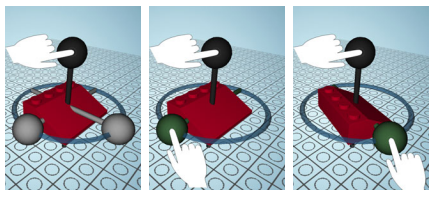
\includegraphics[width=.48\textwidth]{figure/ltouchit.png}
    }
    \hspace{0.2em} % 水平间隔
    \subfigure[多点触控方法]{
        \label{fig-4-r}
        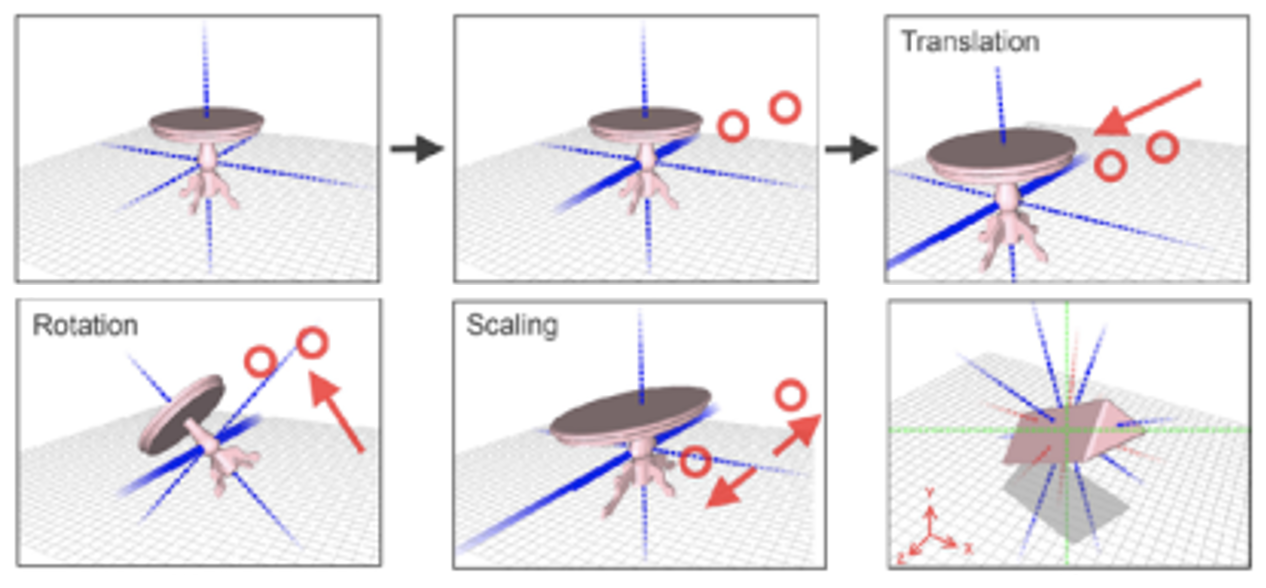
\includegraphics[width=.47\textwidth]{figure/multi_touch.png}
    }
    \caption{两种基于手部动作(含手柄)追踪的非直接对象操纵方法}
    \label{fig-4}
\end{figure}

另外一种值得一提的基于手部动作追踪的方法是外加虚拟控制柄(见图\ref{fig-3});虽然这类方法暂未被应用到虚拟环境中,但是它们对于对象操纵的研究是颇具启发的。Houde团队在1992年开发了一种基于“操纵盒”的方法;这种方法由一个围绕着物体的边界长方体框组成,拖动长方体即拖动物体,另外还有三个旋转柄用于围绕其中心轴旋转物体\upcite{1992Stephanie}。Conner团队也采用了设置虚拟控制柄来进行对象操纵;他们的方法允许完整的9-DOF(Degree of Freedom,自由度)控制(平移、旋转和缩放)甚至诸如扭曲的其他变形\upcite{1992Conner}。该方法的虚拟控制柄的两端有一个小球体,它们将几何变换约束在一个平面或轴上;用户拖动其中一个球体可以平移、旋转或缩放物体。秉承着这两个方法的思想,Mendes团队在2016年提出了相似的一个基于外加虚拟控制柄的方法。他们从实验结果中提出了一套发展准则:(1)直接操作很适合粗略的变换;(2)位移和旋转操作应尽可能分离,以防止不需要的变换;(3)单一的DOF分离对于精确的变换是非常理想的,通常用于细粒度的调整。

2010年以后,基于手部动作(含手柄)追踪的非直接对象操纵方法开始出现。其中较有代表性的两个方法为Mendes团队在2011年提出的LTouchIt和Kin-Chung Au团队在2012年提出的多点触摸方法(见图\ref{fig-4})。LTouchIt虽然使用了直接操纵平移的方法,但在DOF分离之后,它可以控制物体在不超过两个维度上的位置,并使用旋转手柄一次围绕一个轴进行旋转;用户可以选择一个手柄来定义一个旋转轴,并通过另一只手的操作来指定旋转角度\upcite{2011Mendes}。Au团队利用多点触摸表面的高输入带宽,将标准变换部件的操作能力委托给多点触摸手势。这使得使用单一的多点触控动作就能对约束和变换操作进行无缝控制。用户可以用两个触摸点选择一个候选轴,通过按住并移动两个手指来进行物体的变换\upcite{2012Au}。

目前,基于手部动作(含手柄)的追踪的对象操纵方法的SOTA(state-of-the-art,最先进方法)为Gloumeau团队在2020年提出的PinNPivot方法\upcite{2021Gloumeau}。这个方法使用“销钉(pin)”来约束1DOF/2DOF/3DOF旋转;PinNPivot还支持6DOF操纵和3DOF平移,具体的一个操作流程可参考图\ref{fig-5}。在该团队与以往技术的比较表明,PinNPivot拥有更准确和更快的操纵效率。

\begin{figure}[t!]
    \centering
    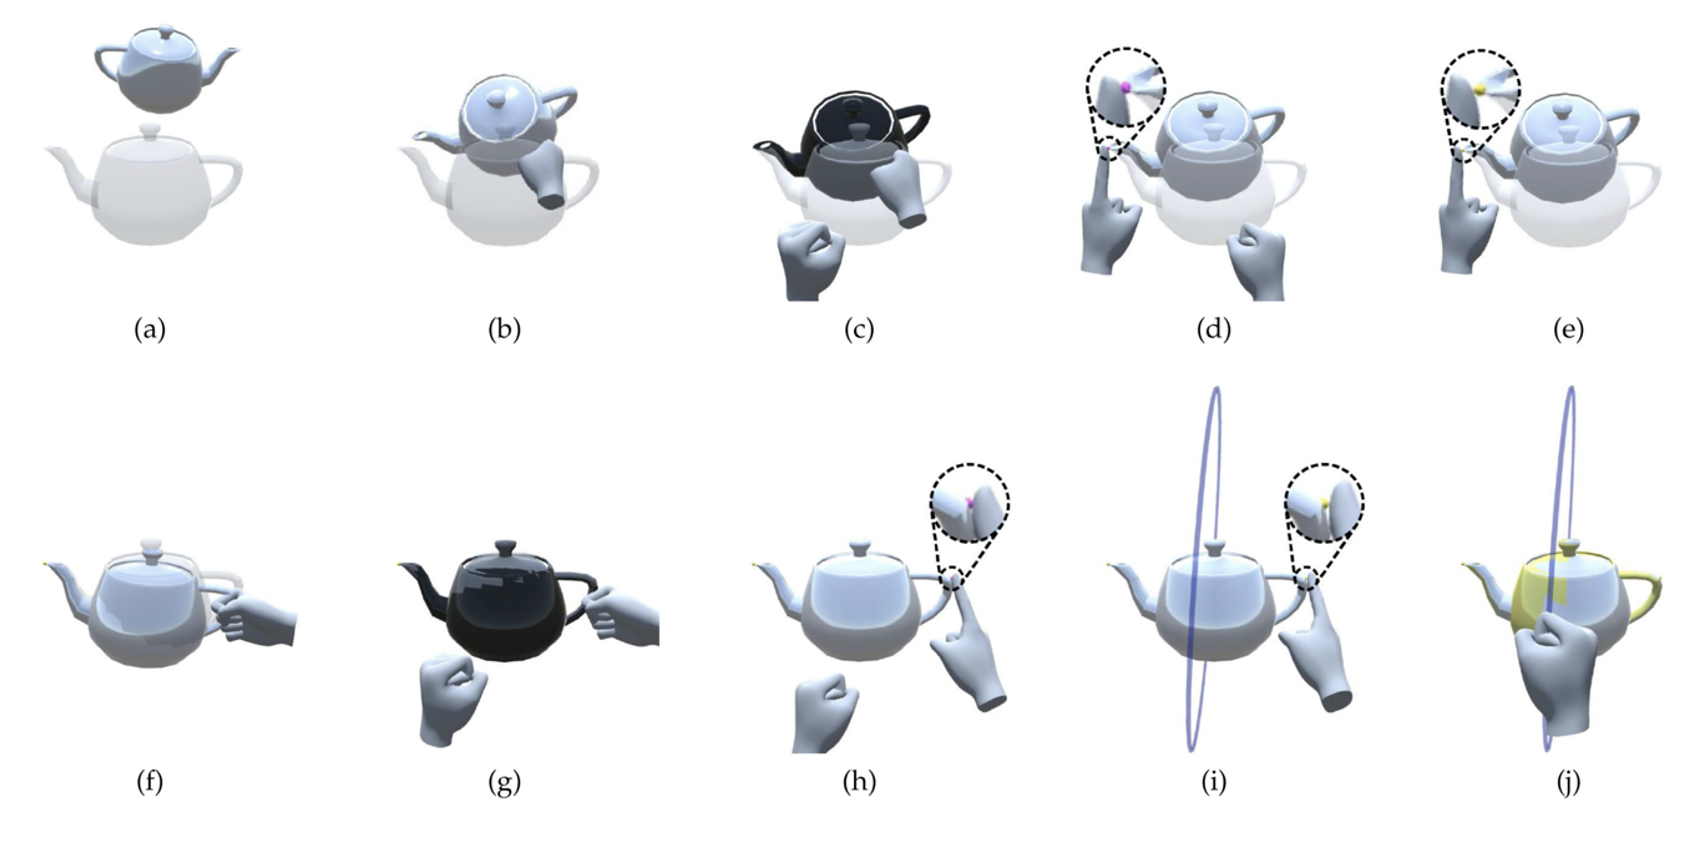
\includegraphics[width=.99\textwidth]{figure/pinnpivot.png}
    \caption{目前基于手部动作(含手柄)的对象操纵最优方法:PinNPivot}
    \label{fig-5}
\end{figure}

\section{基于眼动的操纵}

在2015年以后,眼球追踪在头戴式虚拟现实显示器中的应用越来越多,各种集成了眼球追踪器的头盔已经在市场上销售。根据Adhanom团队在2023年发表的研究,眼动跟踪在虚拟现实中的应用是高度多样化的,并且跨越了多个学科\upcite{2023Adhanom}。因此,近年来基于眼动追踪的对象操纵方法应运兴起。

在VR中实现基于眼睛注视的指向的最常见方法是使用眼动仪提供的3D注视方向向量,并观察场景中的哪些对象与方向向量相交\upcite{2019Sidenmark}。通常,射线是基于方向向量投射的,并且射线相交的第一个物体被认为是被指向的项目(见图\ref{fig-6})。这与射线广播的基本思想是一致的。各种研究表明,基于凝视的指向比基于手的指向更快,因为我们能够比我们的手更快地将目光移向目标\upcite{2000Tanriverdi}。然而,由于眼球运动的固有生理特性和眼动追踪的技术限制,与其他常见的指点界面相比,基于眼睛注视的准确度还是稍显逊色的\upcite{2018Hansen}\upcite{2019Luro}。基于眼睛注视的指向界面中的不准确性主要有两种形式,一是由眼睛跟踪数据中的自然噪声引起的,二是由眼睛跟踪数据质量不稳定引起的。

\begin{figure}[b!]
    \centering
    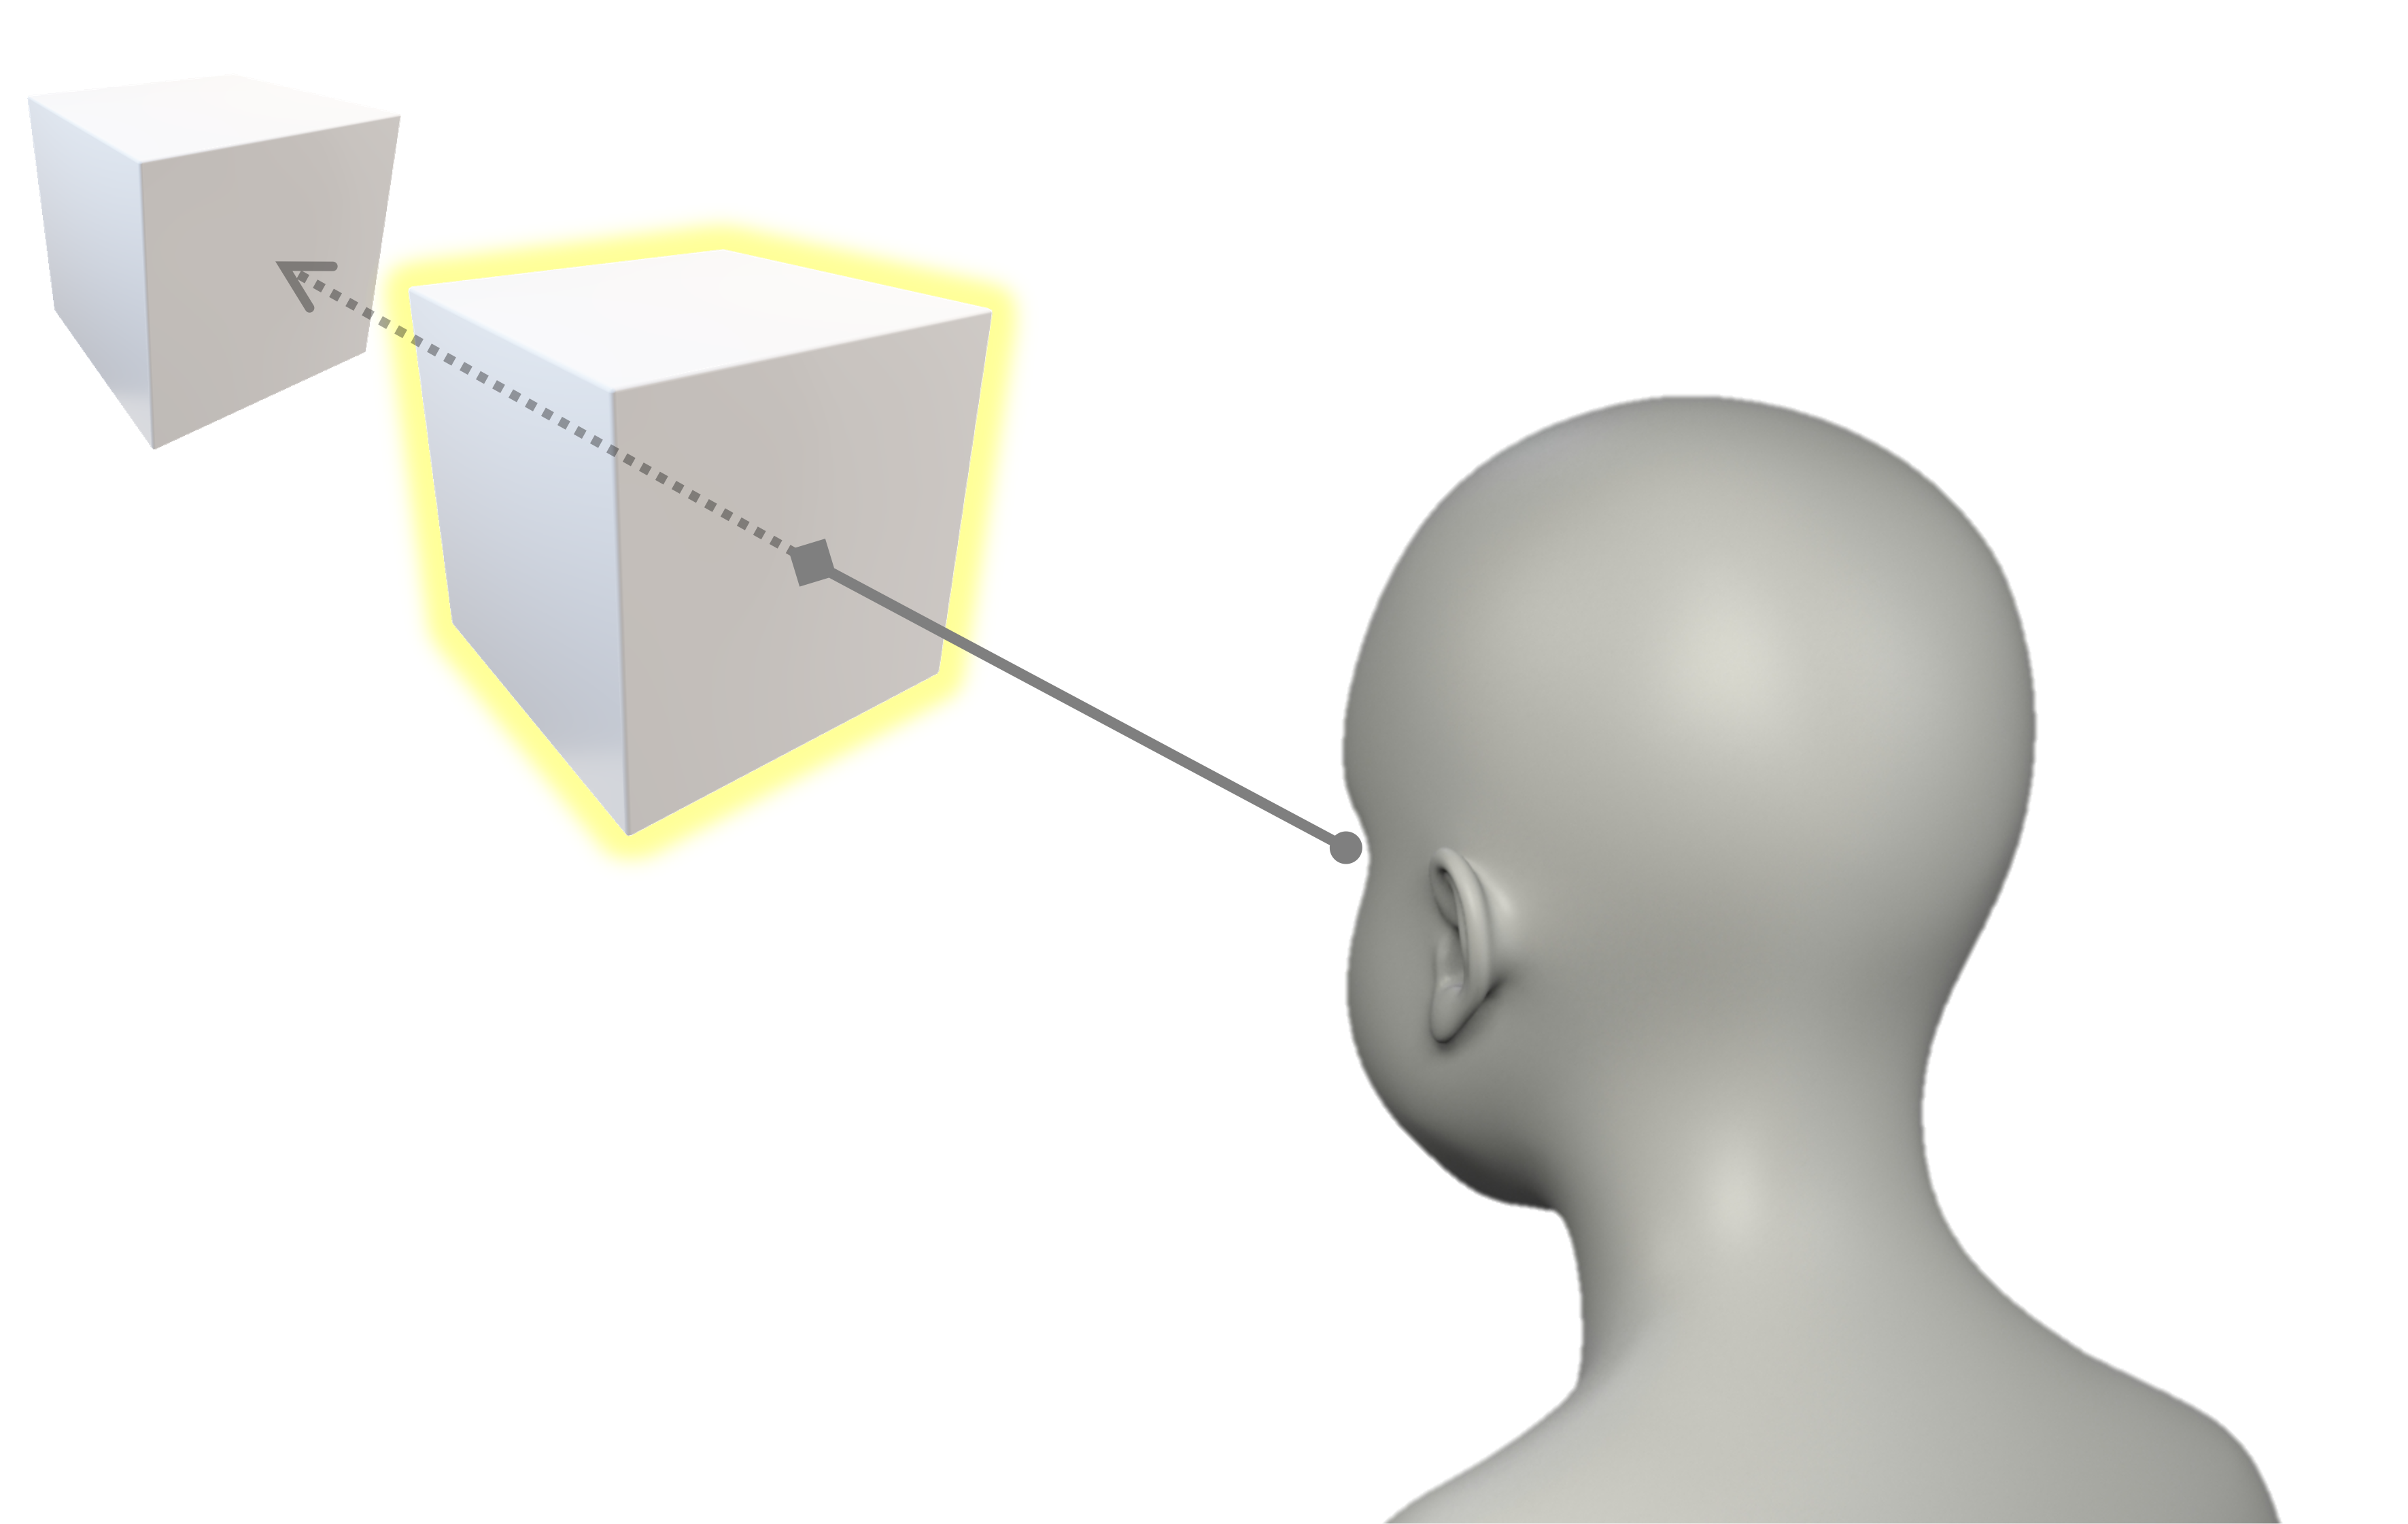
\includegraphics[width=.45\textwidth]{figure/gazing_raycasting.png}
    \caption{基于眼睛注视的指向选择}
    \label{fig-6}
\end{figure}

基于眼动追踪的操纵方法的一大难点是目标对象选择。仅通过眼睛注视进行选择是一项相对具有挑战性的任务,需要实施更为精密的机制以在虚拟环境中使用基于眼睛的交互。根据以往的方法,我们可以实施其他选择确认技术来辅助眼动交互。这样做的一个额外好处是可以解决人机交互领域经典的“点石成金”问题,即“无论你看哪里,都有东西被激活;你不能在没有发出命令的情况下看任何地方”\upcite{1990Jacob}\upcite{2016Jacob}。

\begin{figure}[t!]
    \centering
    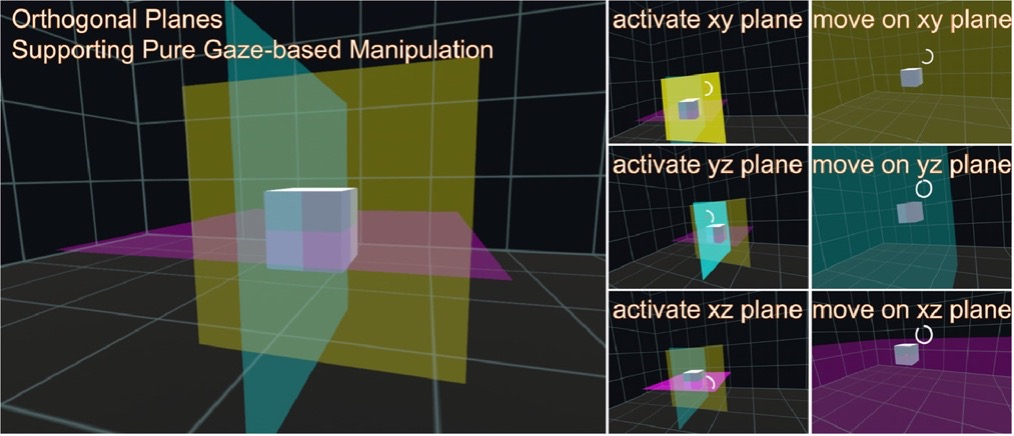
\includegraphics[width=.7\textwidth]{figure/orthogaze.jpg}
    \caption{一个基于眼动和正交平面的对象操纵方法:OrthoGaze}
    \label{fig-7}
\end{figure}

目前已有许多学者使用各种技术来实现虚拟环境中基于注视的交互选择确认。Hansen团队在2018年提出了一种基于眼睛注视的停留进行选择确认的技术\upcite{2018Hansen}。Sidenmark和Gellersen在2019年实施了两种头部辅助的眼动交互技术,第一种是Eye \& Head Dwell,第二种是Eye \& Head Convergence\upcite{2019Sidenmark}。Eye \& Head Dwell是一种停留以确认的技术,其中停留计时器仅由头部支持的凝视转移触发,但可以通过仅眼睛凝视暂停和恢复;Eye \& Head Convergence是一种用于快速目标确认的替代技术,它允许用户通过将眼睛指示器和头部指示器对准目标来确认选择。Kumar和Sharma团队在2016年提出了一种使用眨眼进行选择确认的技术\upcite{2016Kumar}。Pfeuffer团队在2017年提出了一种手眼协统的选择确认方法;这个方法允许用户用眼睛注视物体并同时加以一种“捏合”手势来辅助确认选择\upcite{2017Pfeuffer}。Pai团队在2019年提出了另外一种协同辅助操纵技术;用户可以用目光指向目标,并使用肌电图检测到的手臂肌肉收缩来触发操纵动作\upcite{2019Pai}。Qian和Teather团队在2017年提出了一种通过键盘按钮按下进行选择确认辅助,并使用眼睛注视进行指向选择的方法\upcite{2017Qian}。最近,Sidenmark团队在2020年提出了Outline Pursuits方法,它利用平滑追踪来允许用户在虚拟环境中选择被遮挡的对象\upcite{2020Sidenmark}。

伴随选择技术而来的另外一个值得关注的问题是反馈技术。一个完整的虚拟环境中的对象操纵技术应该向用户提供反馈,让用户能够清楚地了解系统的状态\upcite{2014Majaranta}。由于眼睛对视野中的视觉变化很敏感,它们会本能地尝试将注意力转移到这些视觉变化上。因此,在向用户提供反馈时应该格外小心,因为视觉上突出的反馈机制可能会产生意想不到的后果,即转移用户的视线以产生不期望的交互动作。Boyer团队在2017年提出的一种非视觉反馈方法,他们使用听觉反馈来避免不必要的视线转移\upcite{2017Boyer}。然而,学界依然有很多基于视觉的反馈方法:Blattgerste团队在2018年提出了一种突出显示所选对象的反馈方法;Mohan团队也在2018年提出了一种在所选对象周围显示确认标志的方法;Sidenmark团队在2020年提出了一种在所选对象周围显示轮廓的反馈方法\upcite{2018Blattgerste}\upcite{2018Mohan}\upcite{2020Sidenmark}。

根据目前基于眼动追踪的对象操纵方法的研究数量,眼动追踪将很快成为HMD系统不可或缺的一部分。因此,我们预计围绕HMD眼动追踪的研究和开发将在未来几年加速和扩展。然而,目前大部分眼动追踪方法依旧存在许多值得优化的问题。除了硬件限制,交互动作所带来的生理性不适也需要得到改善。大多数基于眼动追踪的操纵方法都包含眨眼命令(包括眨眼、双眼眨眼和眨眼眼球运动)\upcite{2016Kumar}。要求用户改变他们的自然眨眼频率可能会导致用户眼睛疲劳、眼睛干涩和眼睛疲劳\upcite{2020Hirzle}。Kumar和Sharma团队在2016年的研究结果也表明,频繁眨眼和眨眼会导致用户眼睛疲劳\upcite{2016Kumar}。而且,基于眨眼的界面往往不准确,因为下意识的眨眼很难与自然眨眼区分开来,所以系统往往需要用户做出完全下意识的眨眼动作,如快速多次眨眼。然而,长时间眨眼有明显的缺点,例如减慢交互流程并在长时间眨眼期间阻挡用户的视线。因此,基于眼睛注视的系统控制需要在交互动作上做出合理的优化。

\begin{figure}[b!]
    \centering
    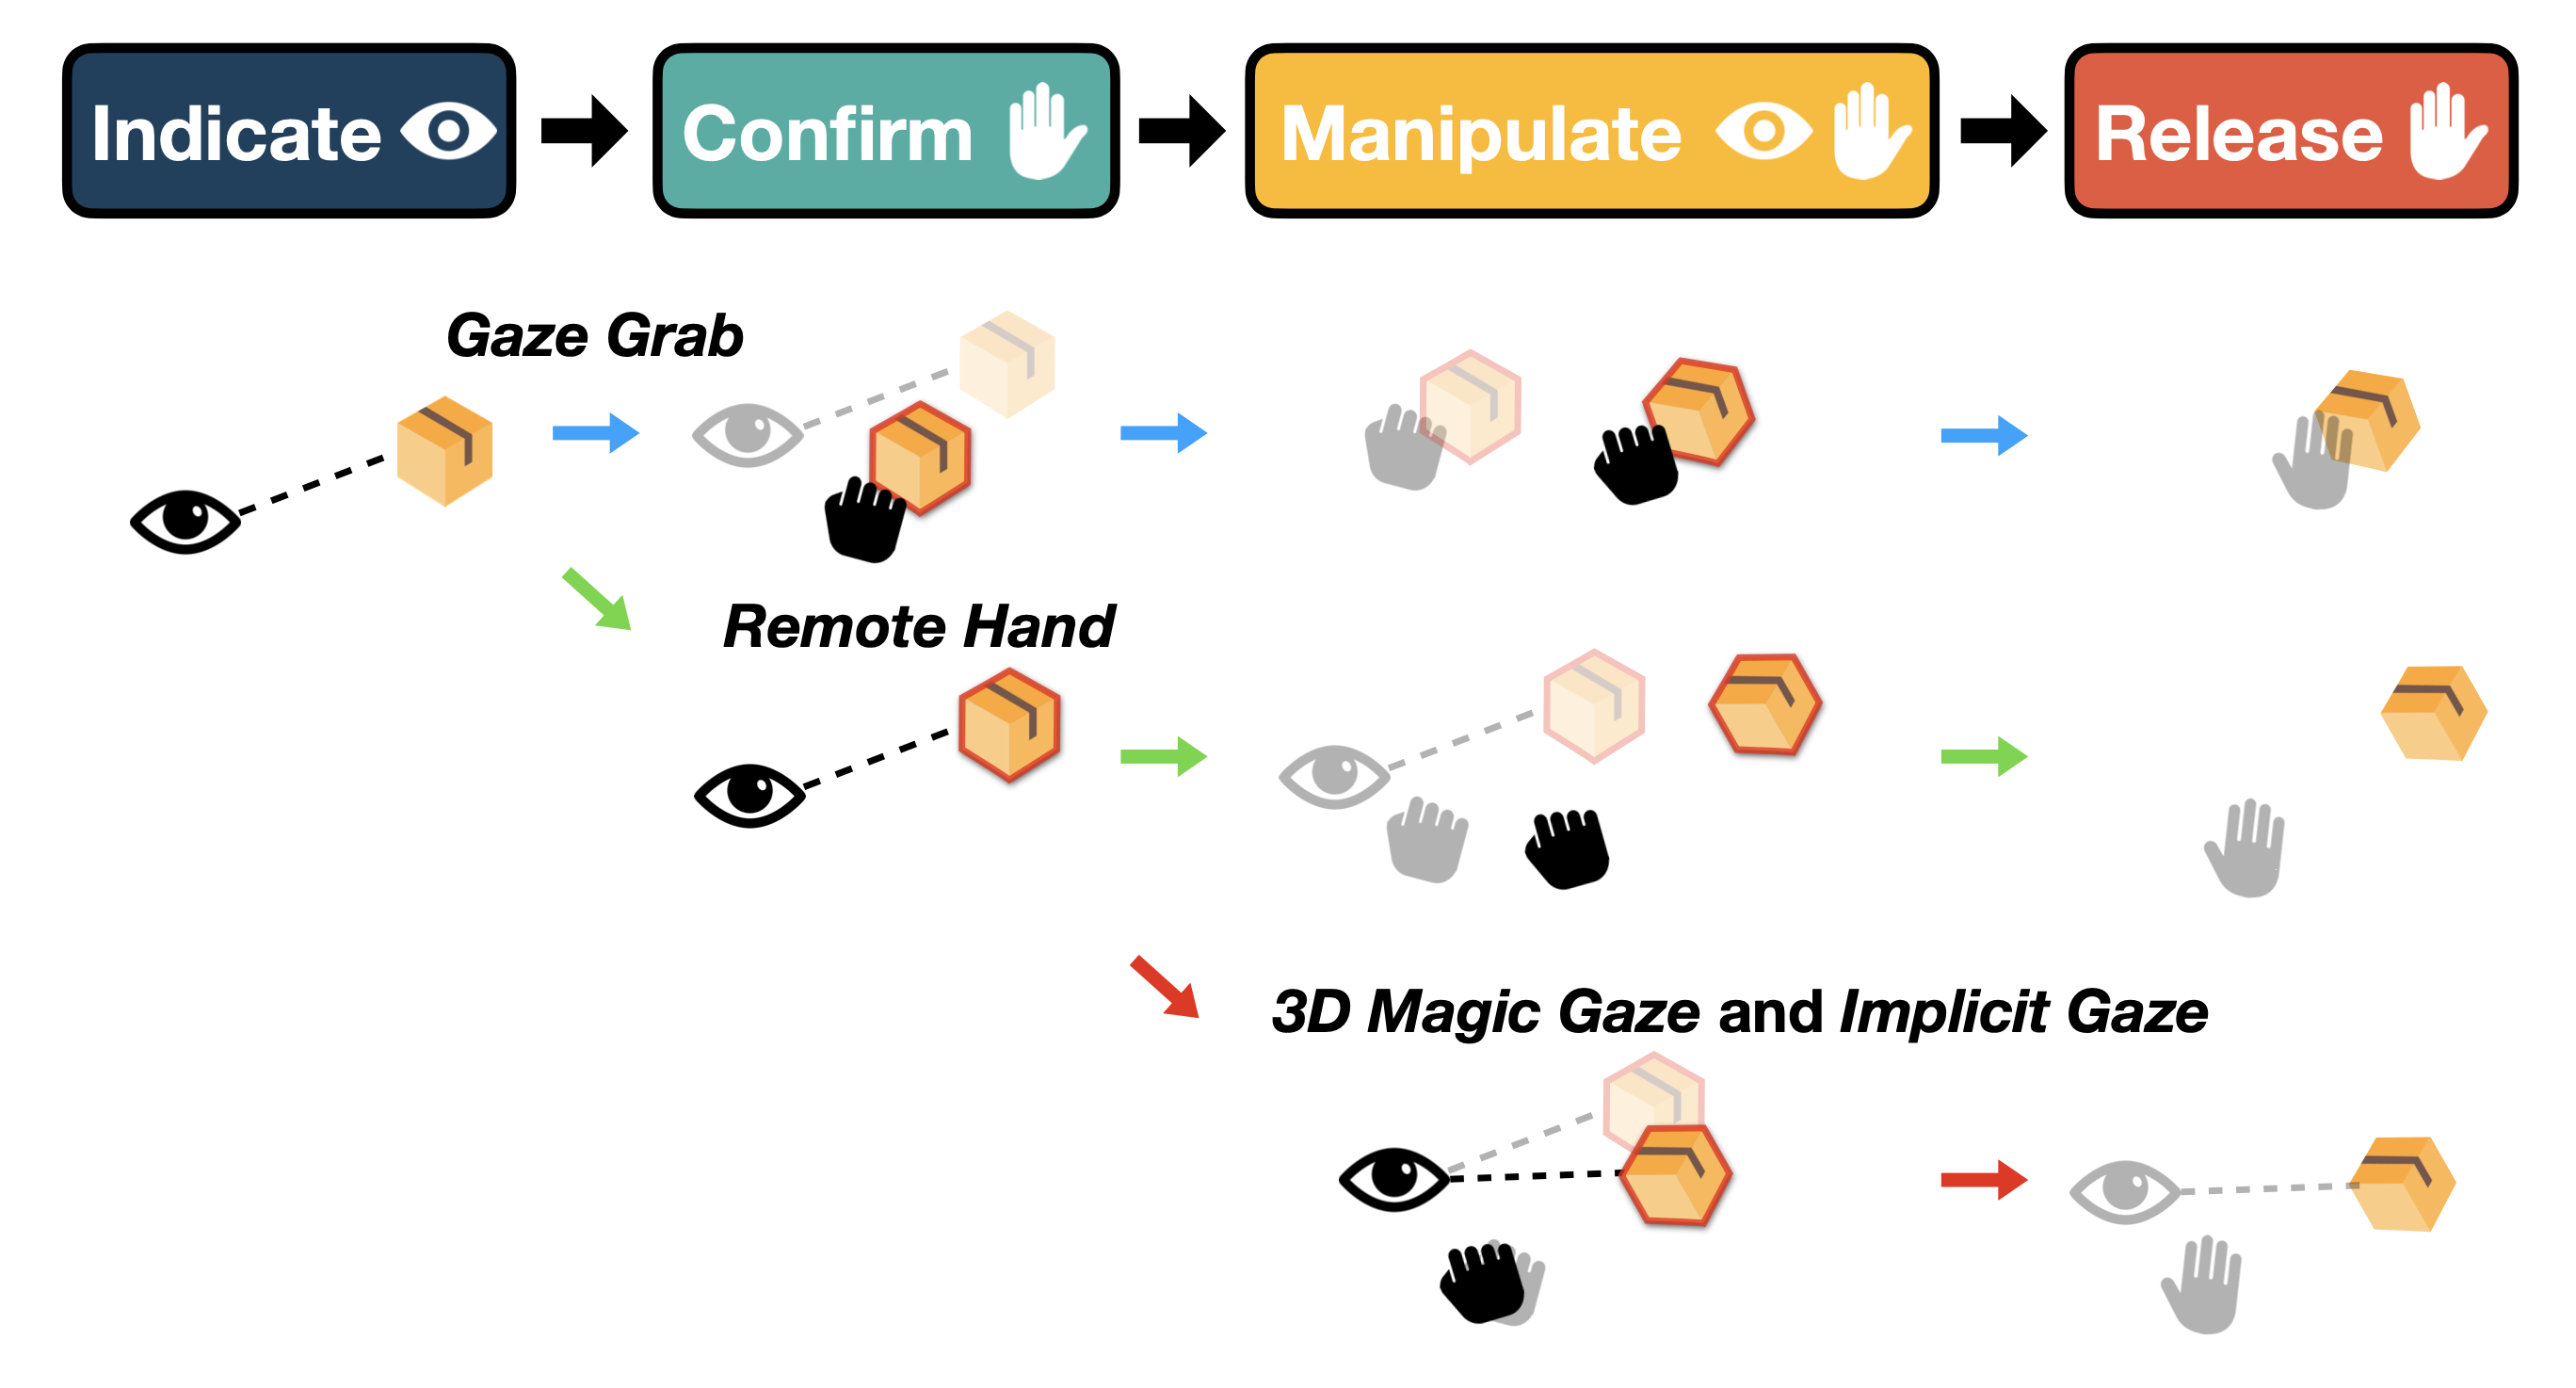
\includegraphics[width=.7\textwidth]{figure/gaze_supported_sota.png}
    \caption{目前涵盖凝视的物体操纵最优方法}
    \label{fig-8}
\end{figure}

目前基于头眼协同的最优方法是Liu团队在2020年提出的OrthoGaze,它允许用户只需用眼睛凝视就能直观地操纵虚拟物体的三维位置(见图\ref{fig-7})\upcite{2020Chang}。该方法利用了三个可选择的正交平面,其中每个平面不仅有助于引导用户在任意虚拟空间中的注视,而且还允许对物体位置进行2DOF操作,是一种完全不依赖手部的对象操纵方法。然而,这个方法仅实现了空间位移,而没有考虑旋转和缩放,所以并不能被视为一个完整的操纵方法。

目前涵盖眼动追踪的对象操纵方法的最优方法为Yu团队在2021年提出的一种基于凝视和手部动作的三维物体操纵方法Implicit Gaze\upcite{2021Yu}。该方法的整个操纵任务可以分解为四个阶段:指示、确认、操作和释放(见图\ref{fig-8})。该研究表明,当所有目标都位于用户前方且在手臂可触及的距离内时,基于凝视的交互对于物体操作没有明显的性能优势;但对于有远处物体的较大空间,凝视输入可以减轻手臂的疲劳问题。眼动和其他模态的不同整合、协调和过渡策略可以为构建更高效的物体操纵技术提供优势。然而,这个方法依旧依靠手部动作,并不能被视为一个完全无手(hands-free)的操纵方法。
